\begin{frame}
    \frametitle{Backwards Induction}
    \centering
    \begin{tikzpicture}[node/.style={draw, circle}]
        \tikzmath{
            let \x1 = 1;
            let \x2 = 5;
            let \y1 = -2.5;
            let \y2 = -5;
        }

        \node[node] (p1_a1) at (0,0) {1};
        \node[node] (p2_a1) at (-2,-1.5) {2};
        \node[node] (p2_a2) at (2,-1.5) {2};
        \node[node] (p1_a2) at (3,-3) {1};

        \node[draw=none] (outcome_1) at (-3,-3) {\( (3,8) \)};
        \node[draw=none] (outcome_2) at (-1,-3) {\( (8,3) \)};
        \node[draw=none] (outcome_3) at (1,-3) {\( (5,5) \)};
        \node[draw=none] (outcome_4) at (2,-4.5) {\( (\underline{2},10) \)};
        \node[draw=none] (outcome_5) at (4,-4.5) {\( (\underline{1},0) \)};

        \draw[->] (p1_a1) -- (p2_a1) node[midway, above] {A};
        \draw[->] (p1_a1) -- (p2_a2) node[midway, above] {B};
        \draw[->] (p2_a1) -- (outcome_1) node[midway, above] {C};
        \draw[->] (p2_a1) -- (outcome_2) node[midway, above] {D};
        \draw[->] (p2_a2) -- (outcome_3) node[midway, above] {E};
        \draw[->] (p2_a2) -- (p1_a2) node[midway, above] {F};
        \draw[->] (p1_a2) -- (outcome_4) node[midway, above] {G};
        \draw[->] (p1_a2) -- (outcome_5) node[midway, above] {H};

        \draw[ultra thin, dashed, red] (\x1, \y1) -- (\x2, \y1);
        \draw[ultra thin, dashed, red] (\x2, \y1) -- (\x2, \y2);
        \draw[ultra thin, dashed, red] (\x2, \y2) -- (\x1, \y2);
        \draw[ultra thin, dashed, red] (\x1, \y2) -- (\x1, \y1);
    \end{tikzpicture}
\end{frame}



\begin{frame}
    \frametitle{Backwards Induction}
    \centering
    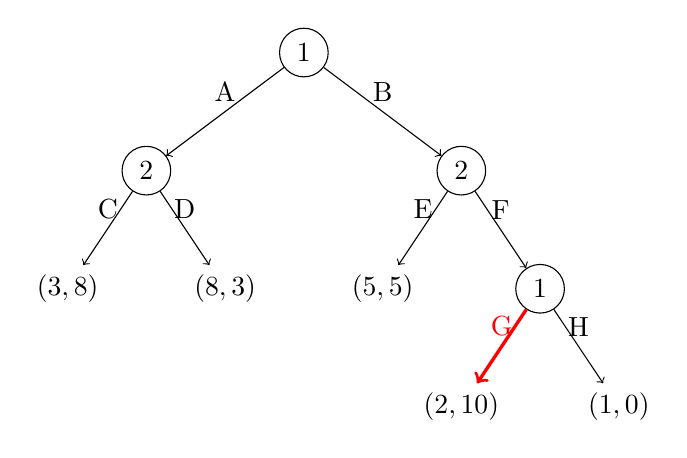
\begin{tikzpicture}[node/.style={draw, circle}]
        \node[node] (p1_a1) at (0,0) {1};
        \node[node] (p2_a1) at (-2,-1.5) {2};
        \node[node] (p2_a2) at (2,-1.5) {2};
        \node[node] (p1_a2) at (3,-3) {1};

        \node[draw=none] (outcome_1) at (-3,-3) {\( (3,8) \)};
        \node[draw=none] (outcome_2) at (-1,-3) {\( (8,3) \)};
        \node[draw=none] (outcome_3) at (1,-3) {\( (5,5) \)};
        \node[draw=none] (outcome_4) at (2,-4.5) {\( (2,10) \)};
        \node[draw=none] (outcome_5) at (4,-4.5) {\( (1,0) \)};

        \draw[->] (p1_a1) -- (p2_a1) node[midway, above] {A};
        \draw[->] (p1_a1) -- (p2_a2) node[midway, above] {B};
        \draw[->] (p2_a1) -- (outcome_1) node[midway, above] {C};
        \draw[->] (p2_a1) -- (outcome_2) node[midway, above] {D};
        \draw[->] (p2_a2) -- (outcome_3) node[midway, above] {E};
        \draw[->] (p2_a2) -- (p1_a2) node[midway, above] {F};
        \draw[->, very thick, red] (p1_a2) -- (outcome_4) node[midway, above] {G};
        \draw[->] (p1_a2) -- (outcome_5) node[midway, above] {H};
    \end{tikzpicture}
\end{frame}


\begin{frame}
    \frametitle{Backwards Induction}
    \centering
    \begin{tikzpicture}[node/.style={draw, circle}]
        \tikzmath{
            let \x1 = 0.4;
            let \x2 = 3.6;
            let \y1 = -1.1;
            let \y2 = -3.2;
        }

        \node[node] (p1_a1) at (0,0) {1};
        \node[node] (p2_a1) at (-2,-1.5) {2};
        \node[node] (p2_a2) at (2,-1.5) {2};
        \node[node] (p1_a2) at (3,-3) {1};

        \node[draw=none] (outcome_1) at (-3,-3) {\( (3,8) \)};
        \node[draw=none] (outcome_2) at (-1,-3) {\( (8,3) \)};
        \node[draw=none] (outcome_3) at (1,-3) {\( (5,\underline{5}) \)};
        \node[draw=none] (outcome_4) at (2,-4.5) {\( (2,\underline{10}) \)};
        \node[draw=none] (outcome_5) at (4,-4.5) {\( (1,0) \)};

        \draw[->] (p1_a1) -- (p2_a1) node[midway, above] {A};
        \draw[->] (p1_a1) -- (p2_a2) node[midway, above] {B};
        \draw[->] (p2_a1) -- (outcome_1) node[midway, above] {C};
        \draw[->] (p2_a1) -- (outcome_2) node[midway, above] {D};
        \draw[->] (p2_a2) -- (outcome_3) node[midway, above] {E};
        \draw[->] (p2_a2) -- (p1_a2) node[midway, above] {F};
        \draw[->, very thick, red] (p1_a2) -- (outcome_4) node[midway, above] {G};
        \draw[->] (p1_a2) -- (outcome_5) node[midway, above] {H};

        \draw[ultra thin, dashed, red] (\x1, \y1) -- (\x2, \y1);
        \draw[ultra thin, dashed, red] (\x2, \y1) -- (\x2, \y2);
        \draw[ultra thin, dashed, red] (\x2, \y2) -- (\x1, \y2);
        \draw[ultra thin, dashed, red] (\x1, \y2) -- (\x1, \y1);
    \end{tikzpicture}
\end{frame}


\begin{frame}
    \frametitle{Backwards Induction}
    \centering
    \begin{tikzpicture}[node/.style={draw, circle}]
        \tikzmath{
            let \x1 = -3.6;
            let \x2 = -0.4;
            let \y1 = -1.1;
            let \y2 = -3.2;
        }

        \node[node] (p1_a1) at (0,0) {1};
        \node[node] (p2_a1) at (-2,-1.5) {2};
        \node[node] (p2_a2) at (2,-1.5) {2};
        \node[node] (p1_a2) at (3,-3) {1};

        \node[draw=none] (outcome_1) at (-3,-3) {\( (3,\underline{8}) \)};
        \node[draw=none] (outcome_2) at (-1,-3) {\( (8,\underline{3}) \)};
        \node[draw=none] (outcome_3) at (1,-3) {\( (5,5) \)};
        \node[draw=none] (outcome_4) at (2,-4.5) {\( (2,10) \)};
        \node[draw=none] (outcome_5) at (4,-4.5) {\( (1,0) \)};

        \draw[->] (p1_a1) -- (p2_a1) node[midway, above] {A};
        \draw[->] (p1_a1) -- (p2_a2) node[midway, above] {B};
        \draw[->] (p2_a1) -- (outcome_1) node[midway, above] {C};
        \draw[->] (p2_a1) -- (outcome_2) node[midway, above] {D};
        \draw[->] (p2_a2) -- (outcome_3) node[midway, above] {E};
        \draw[->, very thick, red] (p2_a2) -- (p1_a2) node[midway, above] {F};
        \draw[->, very thick, red] (p1_a2) -- (outcome_4) node[midway, above] {G};
        \draw[->] (p1_a2) -- (outcome_5) node[midway, above] {H};

        \draw[ultra thin, dashed, red] (\x1, \y1) -- (\x2, \y1);
        \draw[ultra thin, dashed, red] (\x2, \y1) -- (\x2, \y2);
        \draw[ultra thin, dashed, red] (\x2, \y2) -- (\x1, \y2);
        \draw[ultra thin, dashed, red] (\x1, \y2) -- (\x1, \y1);
    \end{tikzpicture}
\end{frame}


\begin{frame}
    \frametitle{Backwards Induction}
    \centering
    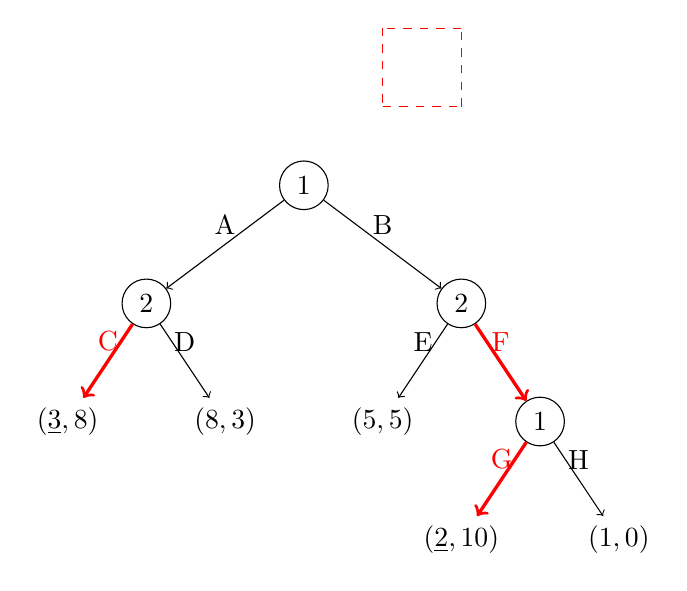
\begin{tikzpicture}[node/.style={draw, circle}]
        \tikzmath{
            let \x1 = -2.5;
            let \x2 = 2.5;
            let \y1 = 0.5;
            let \y2 = -1.75;
        }

        \node[node] (p1_a1) at (0,0) {1};
        \node[node] (p2_a1) at (-2,-1.5) {2};
        \node[node] (p2_a2) at (2,-1.5) {2};
        \node[node] (p1_a2) at (3,-3) {1};

        \node[draw=none] (outcome_1) at (-3,-3) {\( (\underline{3},8) \)};
        \node[draw=none] (outcome_2) at (-1,-3) {\( (8,3) \)};
        \node[draw=none] (outcome_3) at (1,-3) {\( (5,5) \)};
        \node[draw=none] (outcome_4) at (2,-4.5) {\( (\underline{2},10) \)};
        \node[draw=none] (outcome_5) at (4,-4.5) {\( (1,0) \)};

        \draw[->] (p1_a1) -- (p2_a1) node[midway, above] {A};
        \draw[->] (p1_a1) -- (p2_a2) node[midway, above] {B};
        \draw[->, very thick, red] (p2_a1) -- (outcome_1) node[midway, above] {C};
        \draw[->] (p2_a1) -- (outcome_2) node[midway, above] {D};
        \draw[->] (p2_a2) -- (outcome_3) node[midway, above] {E};
        \draw[->, very thick, red] (p2_a2) -- (p1_a2) node[midway, above] {F};
        \draw[->, very thick, red] (p1_a2) -- (outcome_4) node[midway, above] {G};
        \draw[->] (p1_a2) -- (outcome_5) node[midway, above] {H};

        \draw[ultra thin, dashed, red] (\x1, \y1) -- (\x2, \y1);
        \draw[ultra thin, dashed, red] (\x2, \y1) -- (\x2, \y2);
        \draw[ultra thin, dashed, red] (\x2, \y2) -- (\x1, \y2);
        \draw[ultra thin, dashed, red] (\x1, \y2) -- (\x1, \y1);
    \end{tikzpicture}
\end{frame}


\begin{frame}
    \frametitle{Backwards Induction}
    \centering
    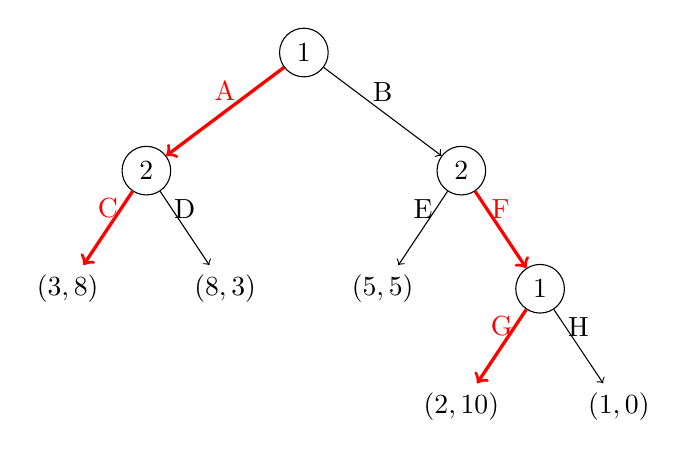
\begin{tikzpicture}[node/.style={draw, circle}]
        \tikzmath{
            let \x1 = -2.5;
            let \x2 = 2.5;
            let \y1 = 0.5;
            let \y2 = -1.75;
        }

        \node[node] (p1_a1) at (0,0) {1};
        \node[node] (p2_a1) at (-2,-1.5) {2};
        \node[node] (p2_a2) at (2,-1.5) {2};
        \node[node] (p1_a2) at (3,-3) {1};

        \node[draw=none] (outcome_1) at (-3,-3) {\( (3,8) \)};
        \node[draw=none] (outcome_2) at (-1,-3) {\( (8,3) \)};
        \node[draw=none] (outcome_3) at (1,-3) {\( (5,5) \)};
        \node[draw=none] (outcome_4) at (2,-4.5) {\( (2,10) \)};
        \node[draw=none] (outcome_5) at (4,-4.5) {\( (1,0) \)};

        \draw[->, very thick, red] (p1_a1) -- (p2_a1) node[midway, above] {A};
        \draw[->] (p1_a1) -- (p2_a2) node[midway, above] {B};
        \draw[->, very thick, red] (p2_a1) -- (outcome_1) node[midway, above] {C};
        \draw[->] (p2_a1) -- (outcome_2) node[midway, above] {D};
        \draw[->] (p2_a2) -- (outcome_3) node[midway, above] {E};
        \draw[->, very thick, red] (p2_a2) -- (p1_a2) node[midway, above] {F};
        \draw[->, very thick, red] (p1_a2) -- (outcome_4) node[midway, above] {G};
        \draw[->] (p1_a2) -- (outcome_5) node[midway, above] {H};
    \end{tikzpicture}
\end{frame}

% This algorithm yields all Subgame Perfect strategies 